\chapter{实验设计与结果分析}\label{chap:experiment}

\section{实验设置}

本文使用的主要数据来自两个来源。第一部分数据是 OpenR1-Math-220k 上的 $10{,}000$ 条 prompt 抽样结果，来自 Qwen2.5-Math-1.5B base 模型；其中每道题均进行了 $256$ 次重复采样，用于估计 prompt 级正确率分布。第二部分数据为同一模型在训练步数 $0,100,\ldots,600$ 的 checkpoint 切片，用于观察训练过程中的分布迁移与信号坍塌变化。

除非特别说明，本文采用如下统计口径：若某题在 $256$ 次采样中答对 $k$ 次，则其经验正确率记为 $\hat p_x=k/256$。随后用 $\hat p_x$ 估计固定组大小下的全对/全错概率，并据此计算不同采样策略的 signal collapse 风险。

\section{Prompt 难度分布统计}

表~\ref{tab:dist_summary} 汇总了 $10{,}000$ 条样本的总体难度分布。可以看到，该数据切片并不是围绕单一中间难度聚集，而是同时包含大量低成功率 prompt 与较长的高成功率尾部。这一结构意味着：若使用固定小组采样，训练中既会频繁遇到“全错组”，也会在后期逐步出现“全对组”。

\begin{table}[!htbp]
    \bicaption{OpenR1-Math-220k 抽样数据的 prompt 正确率统计摘要}{Summary statistics of prompt accuracy on the sampled OpenR1-Math-220k slice.}
    \label{tab:dist_summary}
    \centering
    \small
    \begin{tabular}{lc}
        \hline
        统计量 & 数值 \\
        \hline
        平均正确率 & 0.2623 \\
        中位数正确率 & 0.1055 \\
        标准差 & 0.3133 \\
        非零正确率样本占比 & 81.54\% \\
        正确率恰为 $0$ 的样本占比 & 18.46\% \\
        正确率恰为 $1$ 的样本占比 & 0.56\% \\
        $P_{25}$ & 0.0078 \\
        $P_{75}$ & 0.4609 \\
        $P_{90}$ & 0.8164 \\
        \hline
    \end{tabular}
\end{table}

进一步按桶统计后，正确率位于 $0\sim 8/256$ 的样本占比达到 37.01\%，而 $129/256$ 以上的中高正确率样本占比为 23.15\%。这表明训练语料内部存在显著难度分层，固定预算不可能同时兼顾所有 prompt 的最优采样需求。

图~\ref{fig:prompt_dist} 给出了原始 $10{,}000$ 条样本的双视角分布图。左图展示精确到 $256$ 桶的正确次数直方分布，右图展示归一化后的正确率直方图。可以看到，分布在 $0/256$ 附近存在极高尖峰，而中高正确率区域则呈现较长尾部。这种“左端堆积 + 右端长尾”的结构意味着，如果对所有 prompt 一律采用固定小组采样，那么早期训练会频繁遇到全错组，而后期随着简单题增多，又会逐步积累全对组。

\begin{figure}[!htbp]
    \centering
    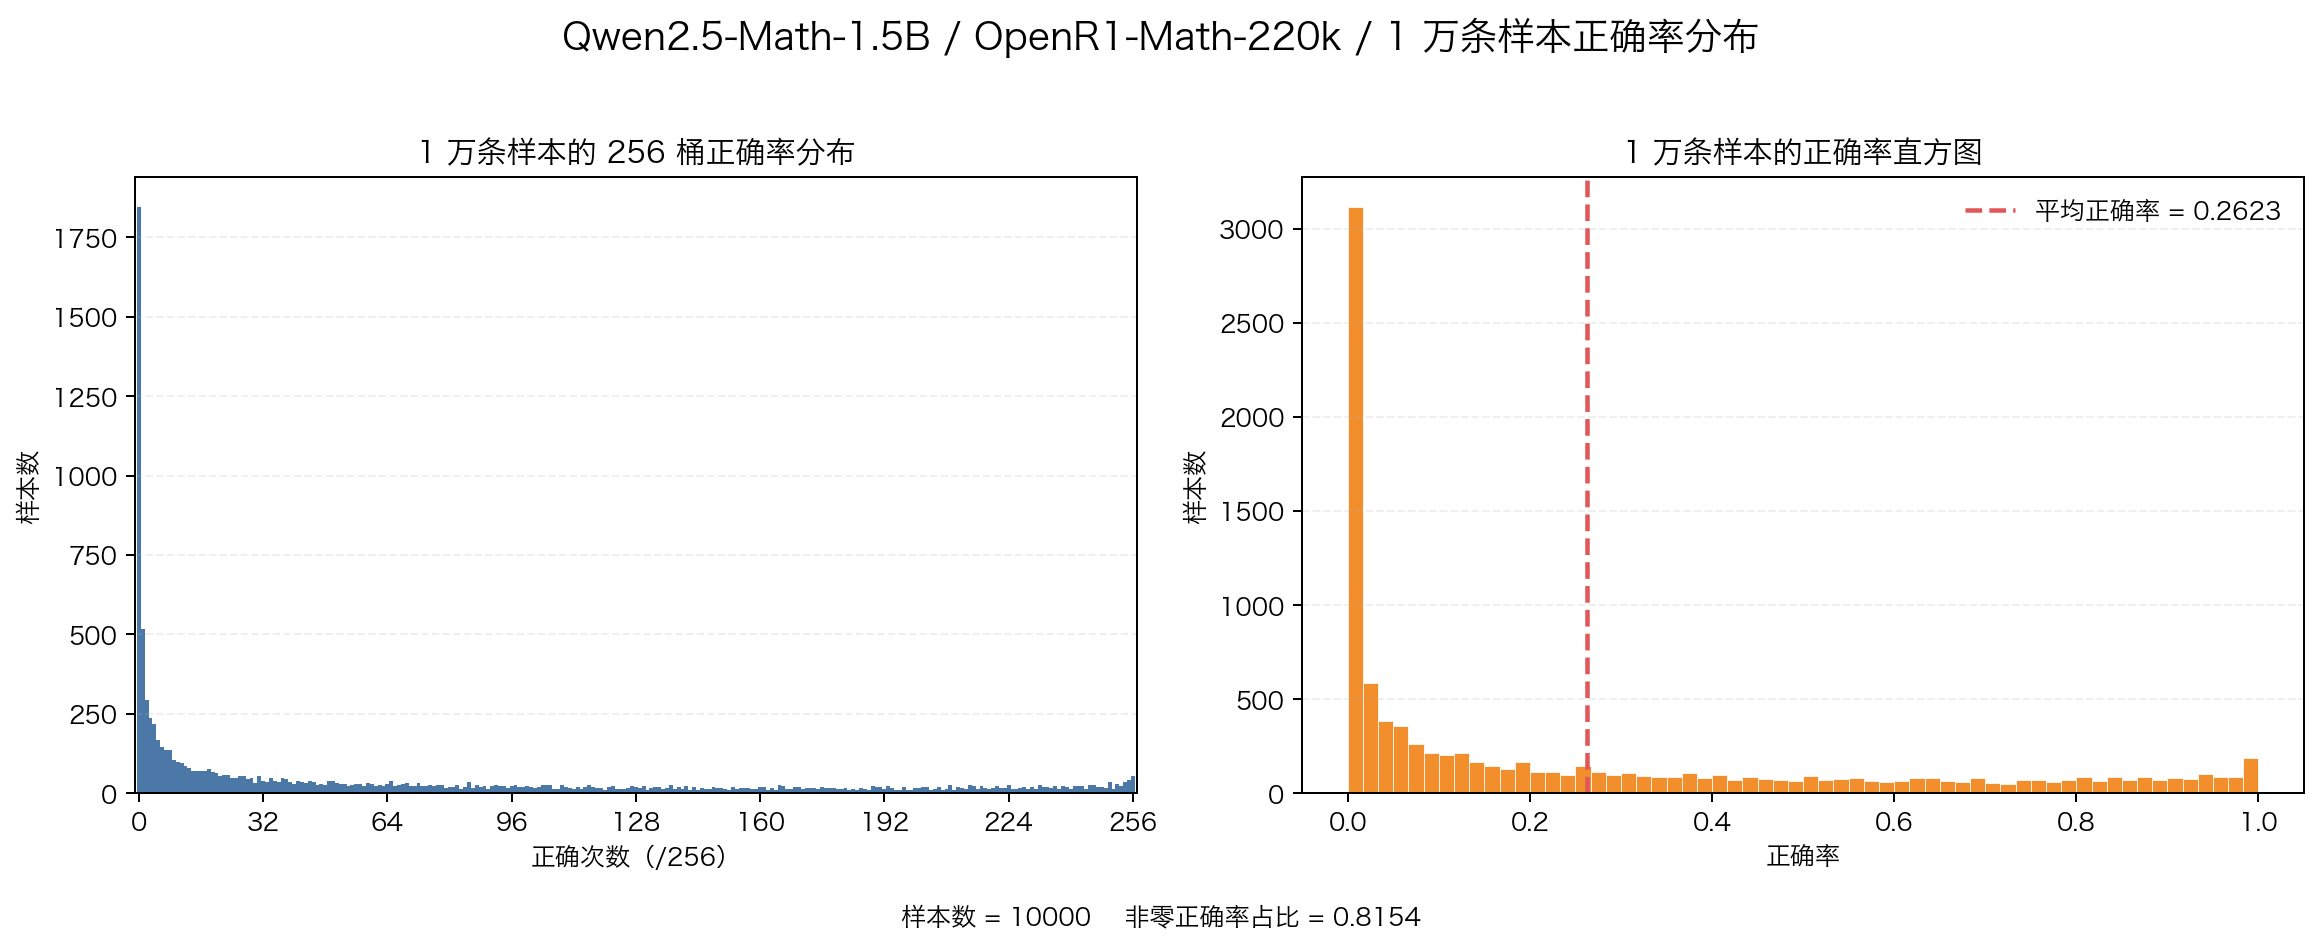
\includegraphics[width=0.95\textwidth]{Img/prompt_accuracy_distribution.png}
    \bicaption{原始样本的 prompt 正确率分布图}{Prompt-level accuracy distribution of the sampled OpenR1-Math-220k slice.}
    \label{fig:prompt_dist}
\end{figure}

\section{信号坍塌的训练前后对比}

基于 prompt 级经验正确率，本文分别估计训练初始点与训练第 600 步时不同组大小下的总体坍塌率。结果如表~\ref{tab:collapse_rate} 所示。可以看到，增大组大小确实会降低全对/全错造成的零信号比例，但即使在 $n=32$ 时，训练初始点仍有 35.36\% 的 prompt 处于坍塌状态；到训练第 600 步，虽然整体正确率上升，坍塌率依然有 26.41\%。

\begin{table}[!htbp]
    \bicaption{训练前后不同组大小下的 signal collapse 概率}{Estimated signal collapse probability under different group sizes before and after training.}
    \label{tab:collapse_rate}
    \centering
    \small
    \begin{tabular}{ccccc}
        \hline
        训练阶段 & $n=4$ & $n=8$ & $n=16$ & $n=32$ \\
        \hline
        Step 0 & 65.35\% & 52.91\% & 43.08\% & 35.36\% \\
        Step 600 & 55.95\% & 41.98\% & 32.75\% & 26.41\% \\
        \hline
    \end{tabular}
\end{table}

这一结果说明两点。首先，所谓零信号并非个别异常样本，而是固定小组采样在真实训练分布上的系统性现象。其次，随着训练推进，虽然“全错”比例下降，但“全对”比例会同步上升，因此坍塌并不会自动消失，而是会以新的形式持续存在。

为了更清楚地说明这一点，表~\ref{tab:collapse_decomp} 进一步将总体坍塌率分解为“全错坍塌”与“全对坍塌”两部分。可以看到，在训练起点，零信号主要由全错主导；但到第 600 步后，随着模型整体能力提升，$n=8,16,32$ 下的全对坍塌分别上升到 11.84\%、7.58\% 和 4.59\%。这表明训练并不是简单消除了坍塌，而是将其来源从“做不出来”逐渐转向“过于容易而缺少负样本”。

\begin{table}[!htbp]
    \bicaption{训练前后 signal collapse 的全错/全对分解}{Decomposition of signal collapse into all-wrong and all-correct events.}
    \label{tab:collapse_decomp}
    \centering
    \small
    \begin{tabular}{ccccccc}
        \hline
        训练阶段 & 指标 & $n=8$ & $n=16$ & $n=32$ \\
        \hline
        Step 0 & 全错坍塌 & 46.48\% & 39.12\% & 32.90\% \\
        Step 0 & 全对坍塌 & 6.43\% & 3.95\% & 2.46\% \\
        Step 600 & 全错坍塌 & 30.14\% & 25.17\% & 21.82\% \\
        Step 600 & 全对坍塌 & 11.84\% & 7.58\% & 4.59\% \\
        \hline
    \end{tabular}
\end{table}

\section{自适应采样策略比较}

本文进一步比较固定预算、固定块自适应与几何块自适应三类策略。比较时分别采用两种退出规则：其一为“有对有错就停”的平衡规则；其二为“只要有对就停”的正样本优先规则。表~\ref{tab:ruleA} 与表~\ref{tab:ruleB} 汇报了在训练全过程上的平均采样成本与信号缺失率。

\begin{table}[!htbp]
    \bicaption{规则 A：有对有错就停时的采样成本与信号缺失率}{Sampling cost and missing-signal rate under Rule A.}
    \label{tab:ruleA}
    \centering
    \small
    \begin{tabular}{lccc}
        \hline
        策略 & 预算序列 & 平均采样数 & 信号缺失率 \\
        \hline
        固定 $8$ 次采样 & $8$ & 8.0000 & 46.02\% \\
        固定 $16$ 次采样 & $16$ & 16.0000 & 36.28\% \\
        固定块自适应 & $4{+}4{+}4{+}4{+}4{+}4{+}4{+}4$ & 15.1211 & 29.36\% \\
        几何块自适应 & $2{+}2{+}4{+}8{+}16$ & 15.4211 & 29.36\% \\
        \hline
    \end{tabular}
\end{table}

\begin{table}[!htbp]
    \bicaption{规则 B：只要有对就停时的采样成本与信号缺失率}{Sampling cost and missing-signal rate under Rule B.}
    \label{tab:ruleB}
    \centering
    \small
    \begin{tabular}{lccc}
        \hline
        策略 & 预算序列 & 平均采样数 & 信号缺失率 \\
        \hline
        固定 $8$ 次采样 & $8$ & 8.0000 & 37.16\% \\
        固定 $16$ 次采样 & $16$ & 16.0000 & 30.74\% \\
        固定块自适应 & $4{+}4{+}4{+}4{+}4{+}4{+}4{+}4$ & 13.2102 & 26.02\% \\
        几何块自适应 & $2{+}2{+}4{+}8{+}16$ & 12.8240 & 26.02\% \\
        \hline
    \end{tabular}
\end{table}

从规则 A 可以看出，自适应采样相较于固定 $16$ 次采样，在平均成本略低的同时将缺失率从 36.28\% 压低到 29.36\%。在规则 B 下，几何块自适应与固定块自适应具有完全一致的缺失率，但平均采样数进一步下降到 12.8240，说明几何块结构并未带来统计层面的明显负担。

若将这种差异写成相对改进幅度，则结论会更加直观。在规则 A 下，固定块自适应相对固定 $16$ 次采样将平均成本降低了 5.49\%，同时将信号缺失率再压低 6.92 个百分点；几何块自适应虽然成本降幅略小，为 3.62\%，但在缺失率上达到完全相同的改善。在规则 B 下，几何块自适应的优势更明显：相对固定 $16$ 次采样，它将平均采样数进一步降低了 19.85\%，同时仍把缺失率从 30.74\% 压低到 26.02\%。这表明在“只要采到正样本即可停止”的预算逻辑下，几何块调度可以同时获得更低成本与更低缺失率。

综合来看，几何块方案的意义不在于对任意指标都绝对占优，而在于它以与固定块几乎相同的统计效果，换来了更加规整的批次组织形式。这种结构化收益为后续 KV Cache 复用与系统并行执行提供了更自然的接口。

\section{训练动态分析}

表~\ref{tab:training_dynamic} 汇总了训练关键阶段的奖励与分位数变化。训练从 step 0 到 step 600，平均奖励由 0.2623 提升至 0.4025，中位数正确率由 0.1055 提升至 0.3750，上四分位由 0.4609 提升至 0.7266，说明整体能力分布持续右移。

\begin{table}[!htbp]
    \bicaption{训练过程中的奖励与分布迁移摘要}{Summary of reward and distribution shift during training.}
    \label{tab:training_dynamic}
    \centering
    \small
    \begin{tabular}{ccccc}
        \hline
        Step & 平均奖励 & $0/256$ 占比 & 中位数 $P_{50}$ & 上四分位 $P_{75}$ \\
        \hline
        0 & 0.2623 & 18.46\% & 0.1055 & 0.4609 \\
        300 & 0.3325 & 11.50\% & 0.2539 & 0.6211 \\
        600 & 0.4025 & 10.69\% & 0.3750 & 0.7266 \\
        \hline
    \end{tabular}
\end{table}

若进一步观察全过程，可以发现训练改进并不是均匀发生在所有难度区间。表~\ref{tab:training_dynamic_full} 给出了每 100 步的奖励、极难样本占比以及中高正确率区间的迁移情况。训练 600 步后，平均奖励相对初始点提升了 53.44\%；$0/256$ 占比从 18.46\% 下降到 10.69\%；而 $150\text{--}220/256$ 区间占比则从 11.55\% 上升到 19.47\%，说明大批样本从“偶尔做对”向“较高稳定度做对”迁移。

\begin{table}[!htbp]
    \bicaption{训练全过程的阶段性分布迁移}{Stage-wise distribution shift during training.}
    \label{tab:training_dynamic_full}
    \centering
    \small
    \begin{tabular}{ccccccc}
        \hline
        Step & Reward & $0/256$ & $\leq 8/256$ & $P_{50}$ & $150\text{--}220/256$ & $220{+}/256$ \\
        \hline
        0 & 0.2623 & 18.46\% & 37.01\% & 0.1055 & 11.55\% & 8.20\% \\
        100 & 0.2786 & 18.45\% & 31.78\% & 0.1445 & 12.01\% & 9.21\% \\
        200 & 0.3031 & 12.57\% & 26.94\% & 0.1992 & 13.07\% & 10.64\% \\
        300 & 0.3325 & 11.50\% & 26.59\% & 0.2539 & 14.77\% & 12.38\% \\
        400 & 0.3606 & 11.50\% & 26.59\% & 0.3047 & 15.35\% & 12.82\% \\
        500 & 0.3833 & 11.37\% & 26.59\% & 0.3438 & 16.94\% & 13.01\% \\
        600 & 0.4025 & 10.69\% & 26.58\% & 0.3750 & 19.47\% & 13.76\% \\
        \hline
    \end{tabular}
\end{table}

这个全过程表格揭示出两个更细的现象。第一，训练前 200 步的主要变化来自左尾收缩，即极难样本大量减少；但 300 步之后，$\leq 8/256$ 的总体占比几乎不再下降，说明最难部分很快进入平台区。第二，后续收益主要表现为中位数与中高正确率区间的持续抬升，即模型在“做得偶尔对”和“做得比较稳”之间发生结构性右移，而不是简单把所有样本都推到极高正确率。这意味着后期训练更需要精细地维持难度梯度，否则简单题上的全对组会越来越多，进一步稀释有效训练信号。

如果进一步与总体奖励提升结合来看，可以发现训练收益与坍塌来源迁移是同步发生的：从 step 0 到 step 600，平均奖励累计提升 53.45\%，说明模型确实在持续学习；但与此同时，step 600 时全对坍塌已分别占到 $n=8,16,32$ 总坍塌量的 28.20\%、23.15\% 和 17.38\%。这意味着后期训练中的零信号并不主要来自“模型什么都做不对”，而越来越来自“简单题已经做得过于稳定”。也正因为如此，后期若仍采用固定预算，额外采样就会越来越多地浪费在已无辨别力的简单 prompt 上。

为了把这一过程可视化，图~\ref{fig:reward_curve} 和图~\ref{fig:checkpoint_overview} 分别给出了训练奖励曲线以及不同 checkpoint 的平滑分布总览。奖励曲线显示训练过程基本单调提升，没有出现明显震荡回退；而 checkpoint 总览图则更清楚地展示了分布形态如何从“极端偏左”逐渐过渡到“中间抬升、右侧增强”。尤其是在 step 300 之后，分布曲线在中高正确率区间逐步抬升，但最左端尖峰并未完全消失，这与表格中“左尾平台化、右侧持续抬升”的判断一致。

\begin{figure}[!htbp]
    \centering
    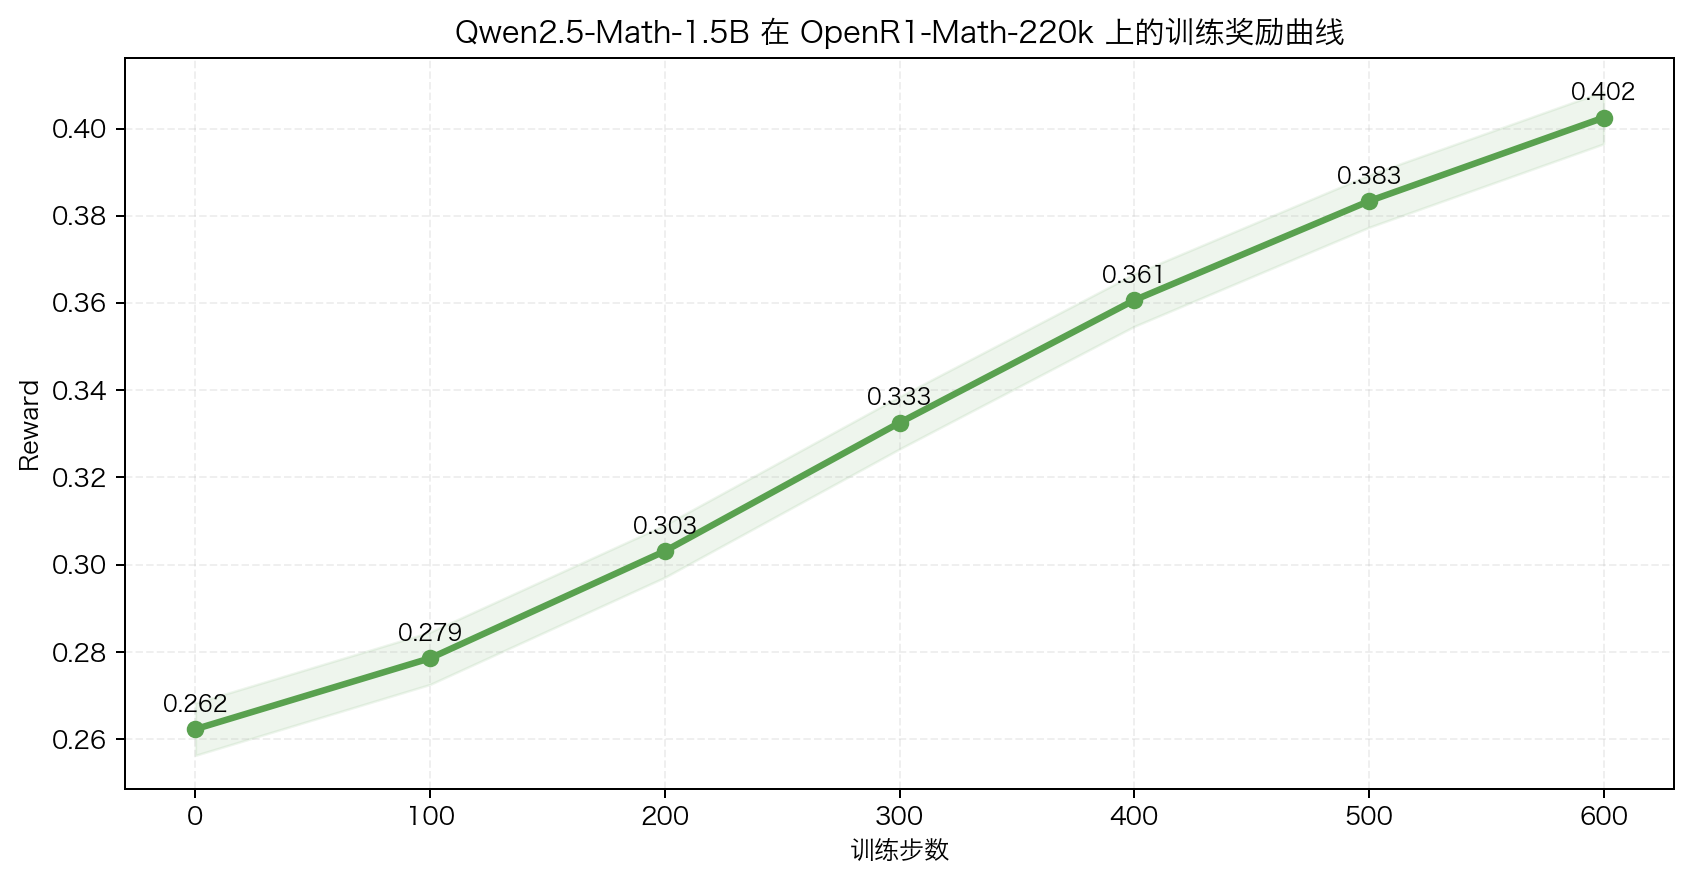
\includegraphics[width=0.82\textwidth]{Img/training_reward_curve.png}
    \bicaption{训练过程中的平均奖励曲线}{Average reward curve during training.}
    \label{fig:reward_curve}
\end{figure}

\begin{figure}[!htbp]
    \centering
    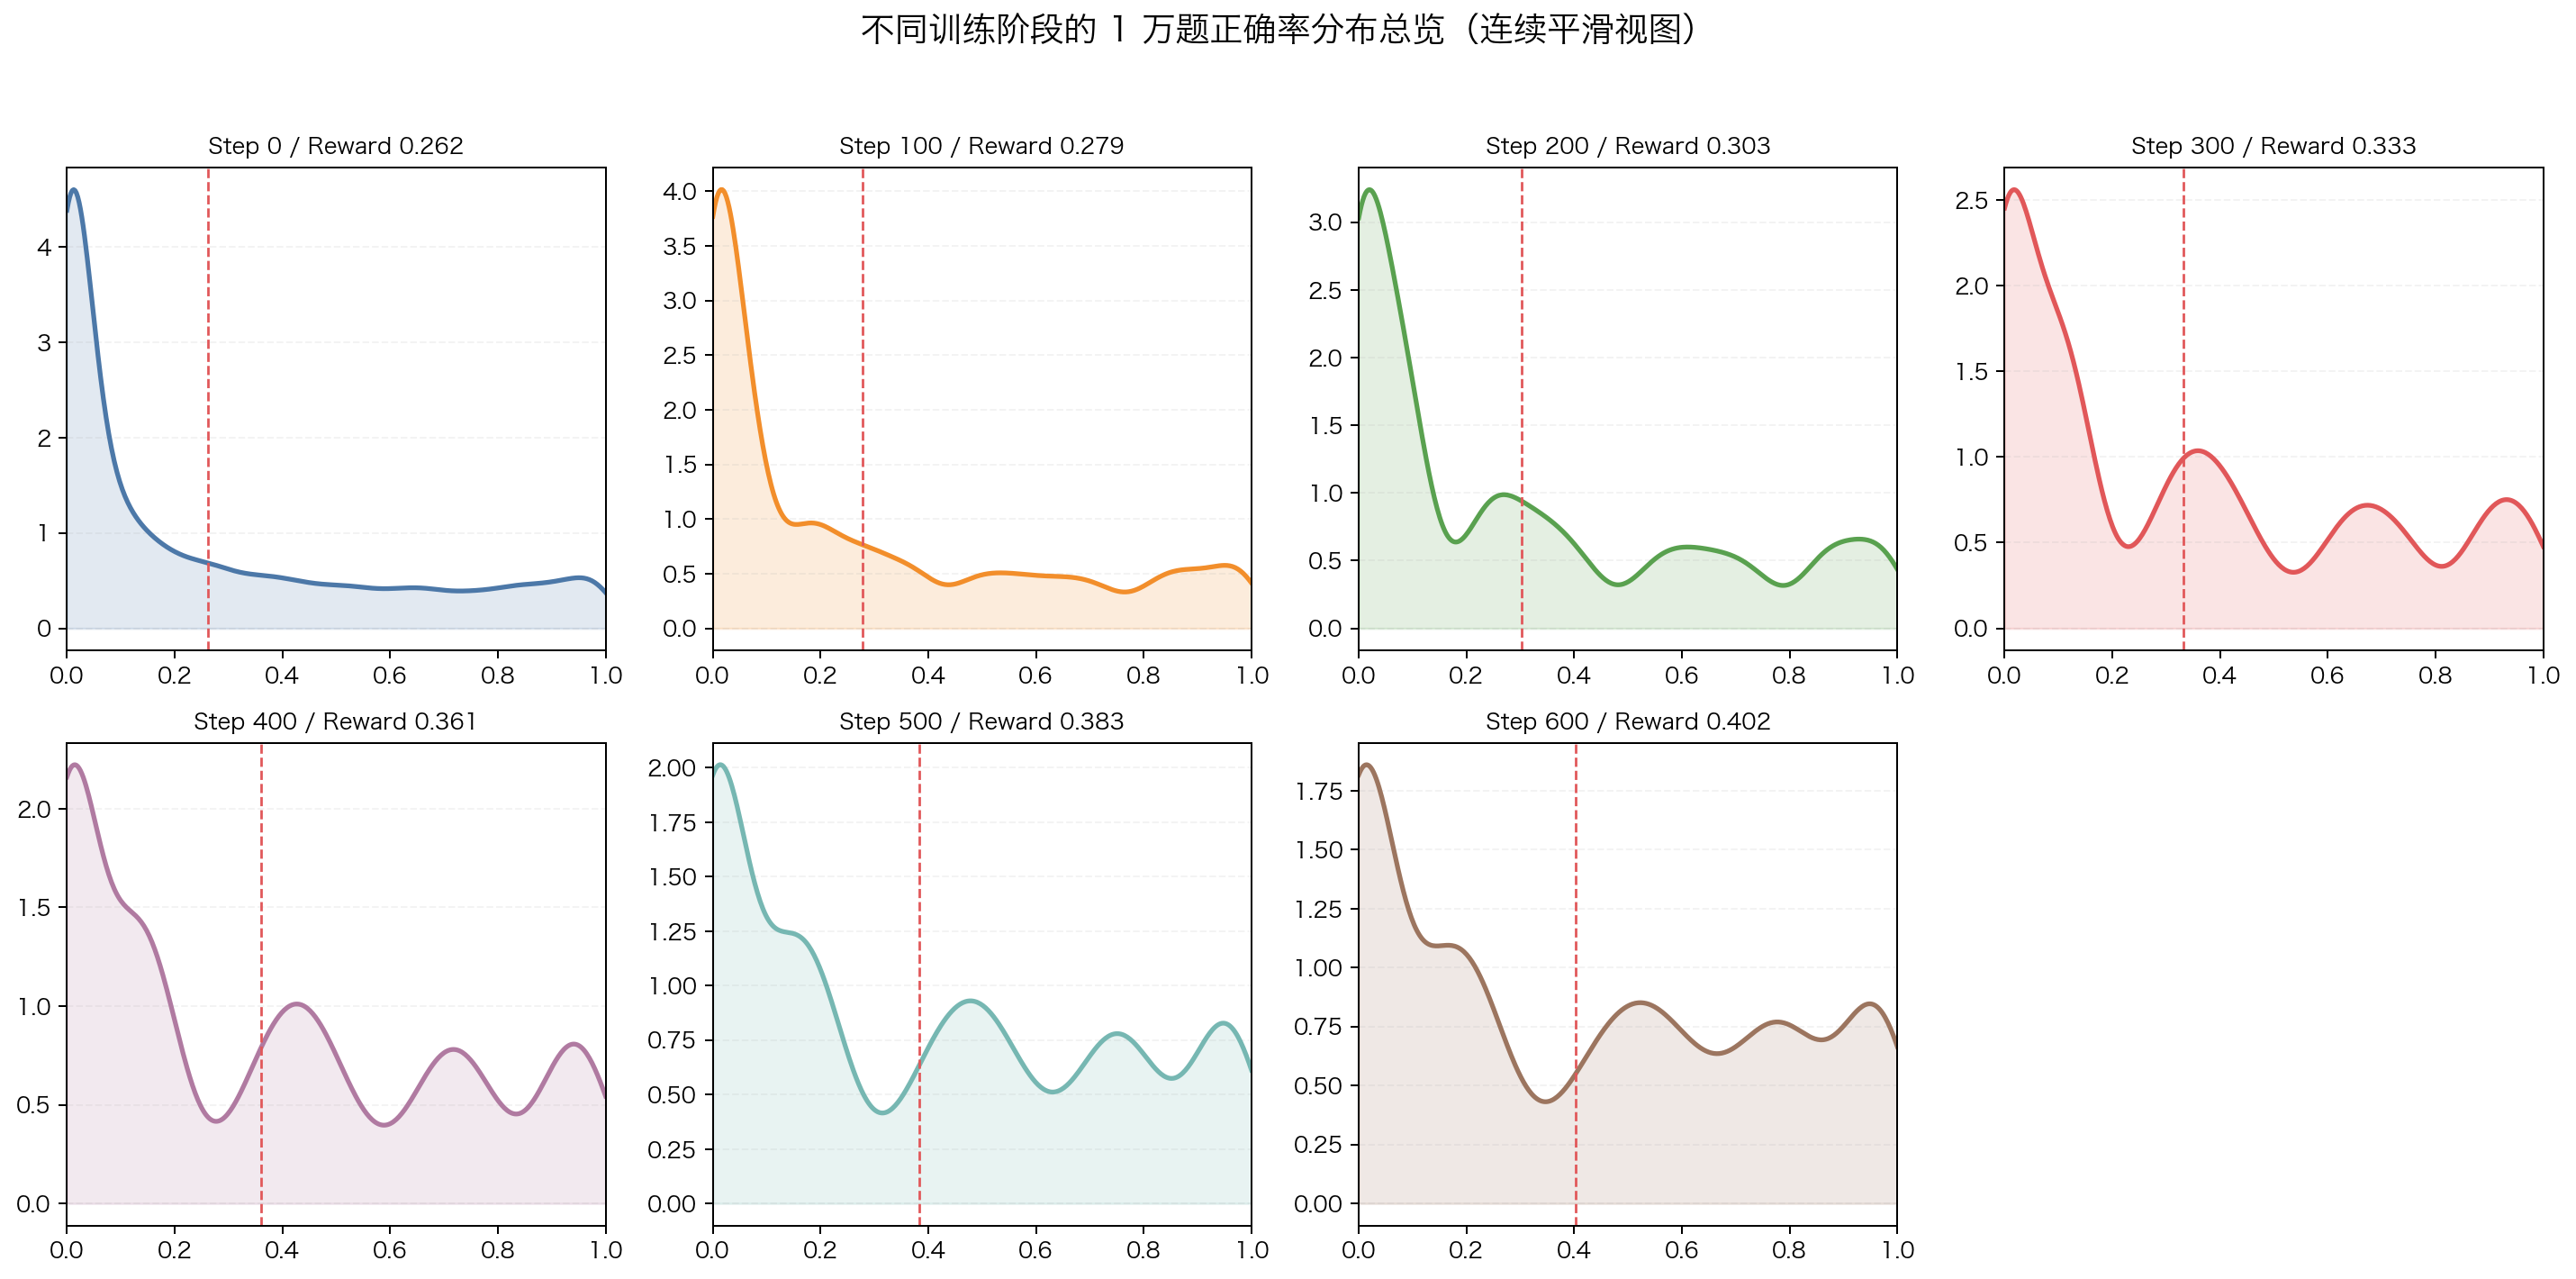
\includegraphics[width=0.98\textwidth]{Img/checkpoint_distribution_overview.png}
    \bicaption{不同 checkpoint 的正确率分布平滑总览}{Smoothed overview of prompt-accuracy distributions across checkpoints.}
    \label{fig:checkpoint_overview}
\end{figure}

值得注意的是，训练后期虽然极低正确率样本比例明显下降，但低端尾部并未完全消失，$0/256$ 的样本占比仍超过 10\%。与此同时，较高正确率区域不断扩张，导致“全对”样本的风险随之上升。换言之，训练动态并不会自然消除 signal collapse，而是将其从“难题全错”逐渐转化为“易题全对”。这正是本文主张采用难度感知采样而非统一固定预算的根本原因。
